\documentclass{beamer}
\usepackage{graphicx}
\usepackage{subfigure}
\usepackage{amsmath,amssymb,amsthm}
\usepackage{mathtools}
\usepackage{epsfig}
\usepackage{color}
\usepackage{geometry}
\usepackage{hyperref}
\usepackage{lmodern}
\usepackage{wrapfig}
\theoremstyle{plain}
\newtheorem{thm}{Theorem}[section]
\theoremstyle{definition}
\newtheorem{exm}[thm]{Example}
\newtheorem{defi}[thm]{Definition}
\newtheorem{lemm}[thm]{Lemma}
\newtheorem{conj}[thm]{Conjecture}
\newtheorem{cond}[thm]{Condition}
\newtheorem{cor}[thm]{Corollary}
\usetheme{Rochester}

\title{Multi-element probabilistic collocation method for sensitivity analysis}
\author{Ryan Viertel}
\institute{University of Utah}
\date{Feb 9, 2015}

\begin{document}

\begin{frame}
\titlepage
\end{frame}

\begin{frame}
\frametitle{Table of Contents}
\tableofcontents
\end{frame}

\AtBeginSection[]
{
    \begin{frame}
    \frametitle{Outline}
    \tableofcontents[currentsection]
    \end{frame}
}

\section{Introduction}

\begin{frame}\frametitle{Introduction}
\begin{itemize}
  \item The ME-PCM is demonstrated in the paper \emph{Multi-element probabilistic collocation method for sensitivity analysis} by Foo et. al. 2008
  \item An alternative to monte-carlo simulations and gradient-based methods for analyzing ODE or PDE system sensitivity.
  \item Has the advantages that:
    \begin{itemize}
     \item It is more computationally efficient 
     \item Can provide a comparison of various output metrics of the system with minimal added computational cost 
     \item Output metrics can be functions of time to allow for sensitivity analysis of a transient response
     \item Utilizes numerical quadrature principles
    \end{itemize}
  \item Can help elucidate and quantify the effects of system parameters
\end{itemize}
\end{frame}

\section{Method}

\begin{frame}\frametitle{ME-PCM Method}
 We will consider a generic system of ODEs
 \begin{equation*}
  \mathbf{x}'(t) = f(\mathbf{x}(t),\mathbf{Y},t)
 \end{equation*}
 Where $\mathbf{x}$ is a vector of system variables, and $\mathbf{Y}$ is a vector of parameters or initial conditions that we will vary. We will consider $\mathbf{Y}$ to be stochastic with a uniform distribution on its domain. There are 3 steps to the ME-PCM:
 \begin{enumerate}
  \item Select a quadrature rule for integration over the parameter space
  \item Select statistical metrics for system output
  \item Sample solutions over parameter space and compute the metrics of system output
 \end{enumerate}
\end{frame}

\section{Application of ME-PCM to example model}

\begin{frame}\frametitle{Model}
 The ME-PCM is applied to a model of chemical signaling for apoptosis.
 \begin{align*}
  x_1' &= -k_1x_4x_1 + k_{d1}x_5\\
  x_2' &= k_{d2}x_5 - k_3x_2x_3 + k_{d3}x_6 + k_{d4}x_6\\
  x_3' &= -k_3x_2x_3 + k_{d3}x_6\\
  x_4' &= k_{d4}x_6 - k_1x_4x_1 - k_{d1}x_5\\
  x_5' &= -k_{d2}x_5 + k_1x_4x_1 - k_{d1}x_5\\
  x_6' &= -k_{d4}x_6 + k_3x_2x_3 - k_{d3}x_6\\
  x_7' &= -k_5x_7x_4 + k_{d5}x_8 + k_{d6}x_8\\
  x_8' &= k_5x_7x_4 - k_{d5}x_8 + k_{d6}x_8\\
 \end{align*}
\end{frame}

\begin{frame}\frametitle{Chemical species of the model}
 \begin{center}
  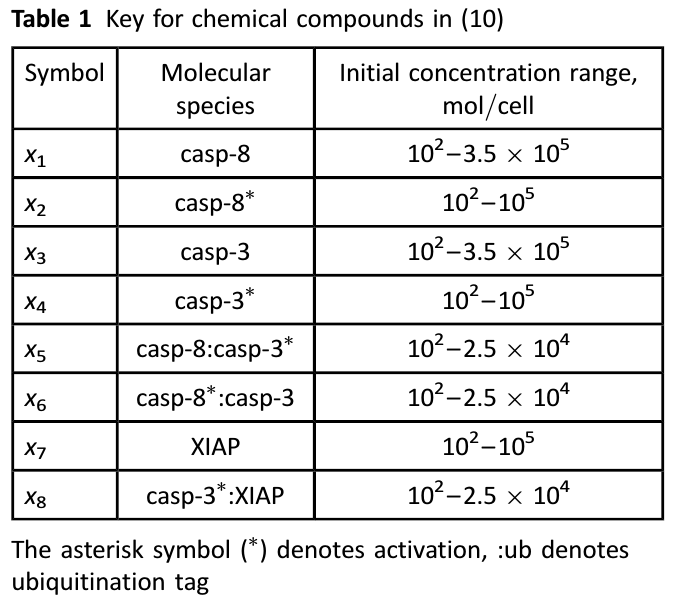
\includegraphics[scale = .35]{table.png}
 \end{center}
\end{frame}



\begin{frame}\frametitle{Select a quadrature rule}
 \begin{itemize}
  \item Discretize parameter space with 10 elements in casp-8* and XIAP ranges, 9 elements in each remaining capsase range, and 1 element in each chemical intermediate range. (This gives 100 elements??)  A sparse Clenshaw-Curtis grid of 317 points per element is selected.
  \begin{center}
   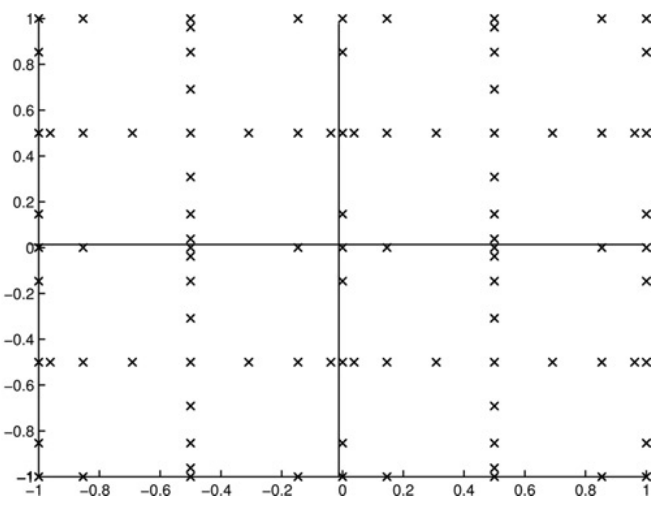
\includegraphics[scale = .25]{clenshaw-curtis.png}
  \end{center}
 \end{itemize}
\end{frame}

\begin{frame}\frametitle{Select statistical metrics for system output}
 Biologically relevant metrics are defined in terms of statistical moments. In this case they chose
 \begin{enumerate}
  \item System sensitivity - The sum of the variance of each molecular species. i.e. $E[x^2] - E[x]^2$ where
  \begin{equation}
   E[x] = \frac{1}{Vol(I)}\int_I{xdx}
  \end{equation}
  \item Species specific sensitivity - the variance of a molecular species
  \item Total exposure - the expected value of the total amount of a molecular species present during the course of the experiment. i.e. $E[f(x)]$ where
  \begin{equation*}
   f(x) = \int_0^t{x(s)ds}
  \end{equation*}
 \end{enumerate}
\end{frame}

\begin{frame}\frametitle{Sample solutions and compute metrics}
 \begin{itemize}
  \item Compute the solution at each sample point in the parameter space.
  \item Compute the value of each metric by integrating over the parameter space on the same grid
  \item For example, the system sensitivity for this example model is given by

  \begin{equation*}
   \sum_{j=1}^8\left[{\left(\frac{1}{Vol(B^i)}\sum_{k=1}^r{x^2_j(t,q_k^i)w_k^i}\right) - \left(\frac{1}{Vol(B^i)}\sum_{k=1}^r{x_j(t,q_k^i)w_k^i}\right)^2}\right]
  \end{equation*}
 \end{itemize}
\end{frame}

\section{Results}

\section{Discussion}

\begin{frame}\frametitle{Discussion}
 \begin{itemize}
  \item The ME-PCM can be used to aid in experimental design and validate/invalidate models by producing falsifiable predictions. For example, the time-varying version can be used to predict the time at which a system should be perturbed in order to modify the outcome.
  \item The ME-PCM is very general, allowing users to define metrics relevant to the specific system being analyzed. The only restriction on these user-defined metrics is that they be integrable functions over the parameter space. Further output metrics can be computed at any time step allowing for an analysis of parameter values on the transient response.
 \end{itemize}
\end{frame}

\begin{frame}\frametitle{Discussion}
 \begin{itemize}
  \item In the limit as the sample element size goes to zero, the variance of a quantity computed with the ME-PCM converges to the magnitude of the square of the gradient of that quantity (normalized by a factor)
  \item The ME-PCM is more computationally efficient by orders of magnitude compared to Monte Carlo methods. Further it is more robust to physical singularities and boundary errors than gradient-based methods and more computationally efficient in its post-processing step.
 \end{itemize}
\end{frame}

\end{document} 